% template created by: Russell Haering. arr. Joseph Crop
\documentclass[12pt,letterpaper]{article}
\usepackage{anysize}
\usepackage{graphicx}
\usepackage{enumerate}
\marginsize{2cm}{2cm}{1cm}{1cm}


\usepackage{listings}

\begin{document}

\begin{titlepage}
    \vspace*{4cm}
    \begin{flushright}
    {\huge
        ECE 375 Pre-Lab 6\\[1cm]
    }
    {\large
     	 External Interrupts
    }
    \end{flushright}
    \begin{flushleft}
    Lab Time: Thursday 10:00 - 11:50
    \end{flushleft}
    \begin{flushright}
    Jeremy Fischer
    
    \vfill
    \rule{5in}{.5mm}\\
    TA Signature
    \end{flushright}

\end{titlepage}


\section{Pre-Lab}

	\begin{enumerate}
		\item
		\textit{In computing, there are traditionally two ways for a microprocessor to listen to other devices and communicate: polling and interrupts. 
		Give a concise overview/description of each method, and give a few examples of situations where you would want to choose one method over the other.}
	
		Polling is when the microcontroller continuously asks the external (or internal) device if it has anything to share with it.
		This takes up time because the processor is busily polling the device for new information.
		Situations where you would want to use the polling method is when the data that the microcontroller needs from the device is changing frequently.
		Interrupts put the responsibility to start a conversation between the device and the microcontroller in the hands of the device.
		The device is responsible for requesting that the microcontroller stop what it's doing and service the request, because a condition has been met.
		Situations where interrupts are used is when the triggering condition isn't met frequently.
		


		
		\item 
		\textit{Describe the function of each bit in the following ATmega128 I/O registers: EICRA, EICRB, and EIMSK. 
		\textbf{Do not} just give a brief summary of these registers; give specific details for each bit of each register, such as its possible values and what function or setting results from each of those values. 
		Also, \textbf{do not} just directly paste your answer from the datasheet, but instead try to describe these details in your own words.}
	
	\textbf{EICRA}
	
		\begin{itemize}
			\item
			EICRA\textsubscript{0}
				
				This bit is paired with EICRA\textsubscript{1}.
				Together they signify if INT0 should be signaled on a falling edge, rising edge, or low level.
			
			\item 
			EICRA\textsubscript{1}
				
				This bit is paired with EICRA\textsubscript{0}.
				Together they signify if INT0 should be signaled on a falling edge, rising edge, or low level.
				Possibilities: 
				\begin{enumerate}
					\item
					EICRA\textsubscript{1} = 1 EICRA\textsubscript{0} = 1 results in INT0 being triggered on a rising edge.
					
					\item
					EICRA\textsubscript{1} = 1 EICRA\textsubscript{0} = 0 results in INT0 being triggered on a falling edge.
					
					\item
					EICRA\textsubscript{1} = 0 EICRA\textsubscript{0} = 0 results in INT0 being triggered on a low level.
				\end{enumerate}
			
			\item
			EICRA\textsubscript{2}
			
			This bit is paired with EICRA\textsubscript{3}.
			Together they signify if INT1 should be signaled on a falling edge, rising edge, or low level.
			
			\item 
			EICRA\textsubscript{3}
			
			This bit is paired with EICRA\textsubscript{2}.
			Together they signify if INT1 should be signaled on a falling edge, rising edge, or low level.
			Possibilities: 
			\begin{enumerate}
				\item
				EICRA\textsubscript{1} = 1 EICRA\textsubscript{0} = 1 results in INT1 being triggered on a rising edge.
				
				\item
				EICRA\textsubscript{1} = 1 EICRA\textsubscript{0} = 0 results in INT1 being triggered on a falling edge.
				
				\item
				EICRA\textsubscript{1} = 0 EICRA\textsubscript{0} = 0 results in INT1 being triggered on a low level.
			\end{enumerate}
			
			
			\item
			EICRA\textsubscript{4}
			
			This bit is paired with EICRA\textsubscript{5}.
			Together they signify if INT2 should be signaled on a falling edge, rising edge, or low level.
			
			\item 
			EICRA\textsubscript{5}
			
			This bit is paired with EICRA\textsubscript{4}.
			Together they signify if INT2 should be signaled on a falling edge, rising edge, or low level.
			Possibilities: 
			\begin{enumerate}
				\item
				EICRA\textsubscript{1} = 1 EICRA\textsubscript{0} = 1 results in INT2 being triggered on a rising edge.
				
				\item
				EICRA\textsubscript{1} = 1 EICRA\textsubscript{0} = 0 results in INT2 being triggered on a falling edge.
				
				\item
				EICRA\textsubscript{1} = 0 EICRA\textsubscript{0} = 0 results in INT2 being triggered on a low level.
			\end{enumerate}
			
				\item
			EICRA\textsubscript{6}
			
			This bit is paired with EICRA\textsubscript{7}.
			Together they signify if INT3 should be signaled on a falling edge, rising edge, or low level.
			
			\item 
			EICRA\textsubscript{7}
			
			This bit is paired with EICRA\textsubscript{6}.
			Together they signify if INT3 should be signaled on a falling edge, rising edge, or low level.
			Possibilities: 
			\begin{enumerate}
				\item
				EICRA\textsubscript{1} = 1 EICRA\textsubscript{0} = 1 results in INT3 being triggered on a rising edge.
				
				\item
				EICRA\textsubscript{1} = 1 EICRA\textsubscript{0} = 0 results in INT3 being triggered on a falling edge.
				
				\item
				EICRA\textsubscript{1} = 0 EICRA\textsubscript{0} = 0 results in INT3 being triggered on a low level.
			\end{enumerate}
			
			
		\end{itemize}

	\textbf{EICRB}

		\begin{itemize}
			\item
			EICRB\textsubscript{0}
			
			This bit is paired with EICRB\textsubscript{1}.
			Together they signify if INT4 should be signaled on a falling edge, rising edge, or low level.
			
			\item 
			EICRB\textsubscript{1}
			
			This bit is paired with EICRB\textsubscript{0}.
			Together they signify if INT4 should be signaled on a falling edge, rising edge, or low level.
			Possibilities: 
			\begin{enumerate}
				\item
				EICRB\textsubscript{1} = 1 EICRB\textsubscript{0} = 1 results in INT4 being triggered on a rising edge.
				
				\item
				EICRB\textsubscript{1} = 1 EICRB\textsubscript{0} = 0 results in INT4 being triggered on a falling edge.
				
				\item
				EICRB\textsubscript{1} = 0 EICRB\textsubscript{0} = 0 results in INT4 being triggered on a low level.
				
				\item
				EICRB\textsubscript{1} = 0 EICRB\textsubscript{0} = 1 results in INT4 being triggered on any level
			\end{enumerate}

			\item
			EICRB\textsubscript{2}
			
			This bit is paired with EICRB\textsubscript{3}.
			Together they signify if INT5 should be signaled on a falling edge, rising edge, or low level.
			
			\item 
			EICRB\textsubscript{3}
			
			This bit is paired with EICRB\textsubscript{2}.
			Together they signify if INT5 should be signaled on a falling edge, rising edge, or low level.
			Possibilities: 
			\begin{enumerate}
				\item
				EICRB\textsubscript{1} = 1 EICRB\textsubscript{0} = 1 results in INT5 being triggered on a rising edge.
				
				\item
				EICRB\textsubscript{1} = 1 EICRB\textsubscript{0} = 0 results in INT5 being triggered on a falling edge.
				
				\item
				EICRB\textsubscript{1} = 0 EICRB\textsubscript{0} = 0 results in INT5 being triggered on a low level.
				
				\item
				EICRB\textsubscript{1} = 0 EICRB\textsubscript{0} = 1 results in INT5 being triggered on any level
			\end{enumerate}
		
			\item
			EICRB\textsubscript{4}
			
			This bit is paired with EICRB\textsubscript{5}.
			Together they signify if INT6 should be signaled on a falling edge, rising edge, or low level.
			
			\item 
			EICRB\textsubscript{5}
			
			This bit is paired with EICRB\textsubscript{4}.
			Together they signify if INT6 should be signaled on a falling edge, rising edge, or low level.
			Possibilities: 
			\begin{enumerate}
				\item
				EICRB\textsubscript{1} = 1 EICRB\textsubscript{0} = 1 results in INT6 being triggered on a rising edge.
				
				\item
				EICRB\textsubscript{1} = 1 EICRB\textsubscript{0} = 0 results in INT6 being triggered on a falling edge.
				
				\item
				EICRB\textsubscript{1} = 0 EICRB\textsubscript{0} = 0 results in INT6 being triggered on a low level.
				
				\item
				EICRB\textsubscript{1} = 0 EICRB\textsubscript{0} = 1 results in INT6 being triggered on any level
			\end{enumerate}
			
			
			\item
			EICRB\textsubscript{6}
			
			This bit is paired with EICRB\textsubscript{7}.
			Together they signify if INT7 should be signaled on a falling edge, rising edge, or low level.
			
			\item 
			EICRB\textsubscript{7}
			
			This bit is paired with EICRB\textsubscript{6}.
			Together they signify if INT7 should be signaled on a falling edge, rising edge, or low level.
			Possibilities: 
			\begin{enumerate}
				\item
				EICRB\textsubscript{1} = 1 EICRB\textsubscript{0} = 1 results in INT7 being triggered on a rising edge.
				
				\item
				EICRB\textsubscript{1} = 1 EICRB\textsubscript{0} = 0 results in INT7 being triggered on a falling edge.
				
				\item
				EICRB\textsubscript{1} = 0 EICRB\textsubscript{0} = 0 results in INT7 being triggered on a low level.
				
				\item
				EICRB\textsubscript{1} = 0 EICRB\textsubscript{0} = 1 results in INT7 being triggered on any level
			\end{enumerate}
		
		
		\end{itemize}


	\textbf{EIMSK}

		\begin{itemize}
			\item
			EIMSK\textsubscript{0}
				
			If EIMSK\textsubscript{0} is set to 0 then INT0 will be ignored.
			If EIMSK\textsubscript{0} is set to 1 then INT0 is allowed to be detected
			
			\item 
			EIMSK\textsubscript{1}
			
			If EIMSK\textsubscript{1} is set to 0 then INT1 will be ignored.
			If EIMSK\textsubscript{1} is set to 1 then INT1 is allowed to be detected
			
			\item
			EIMSK\textsubscript{2}
			
			If EIMSK\textsubscript{2} is set to 0 then INT2 will be ignored.
			If EIMSK\textsubscript{2} is set to 1 then INT2 is allowed to be detected
			
			\item 
			EIMSK\textsubscript{3}
			
			If EIMSK\textsubscript{3} is set to 0 then INT3 will be ignored.
			If EIMSK\textsubscript{3} is set to 1 then INT3 is allowed to be detected
			
			
			\item
			EIMSK\textsubscript{4}
			
			If EIMSK\textsubscript{4} is set to 0 then INT4 will be ignored.
			If EIMSK\textsubscript{4} is set to 1 then INT4 is allowed to be detected
			
			\item 
			EIMSK\textsubscript{5}
			
			If EIMSK\textsubscript{5} is set to 0 then INT5 will be ignored.
			If EIMSK\textsubscript{5} is set to 1 then INT5 is allowed to be detected
			
			\item
			EIMSK\textsubscript{6}
			
			If EIMSK\textsubscript{6} is set to 0 then INT6 will be ignored.
			If EIMSK\textsubscript{6} is set to 1 then INT6 is allowed to be detected
			
			
			\item
			EIMSK\textsubscript{7}
			
			If EIMSK\textsubscript{7} is set to 0 then INT7 will be ignored.
			If EIMSK\textsubscript{7} is set to 1 then INT7 is allowed to be detected
			
		\end{itemize}
	
	
	
		
		\item
		\textit{The ATmega128 microcontroller uses interrupt vectors to execute particular instructions when an interrupt occurs. What is an interrupt vector? 
		List the interrupt vector (address) for each of the following ATmega128 interrupts: Timer/Counter0 Overflow, External Interrupt 5, and Analog Comparator.}
		
		An interrupt vector is what resides in the 32-bits pointed to by the interrupt.
		The interrupt vector contains an instruction to handle the interrupt.
		Usually this is an rcall to the ISR subroutine.
		
		\begin{itemize}
			\item 
			Timer/Counter0 Overflow = \$0020
			
			
			\item 
			External Interrupt 5 = \$000C
			
			
			\item 
			Analog Comparator = \$002E
		\end{itemize}
		
		
		
		
		
		\item 
		\textit{Microcontrollers often provide several different ways of configuring interrupt triggering, such as \textit{level detection} and \textit{edge detection}. 
		Suppose the signal shown in Figure 1 was connected to a microcontroller pin that was configured as an input and had the ability to trigger an interrupt based on certain signal conditions. 
		List the cycles (or range of cycles) for which an external interrupt would be triggered if that pin’s sense control was configured for: (a) rising edge detection, (b) falling edge detection, (c) low level detection, and (d) high level detection. Note: There should be no overlap in your answers, i.e., only one type of interrupt condition can be detected during a given cycle.}
		\begin{figure}[h]
			\centering
			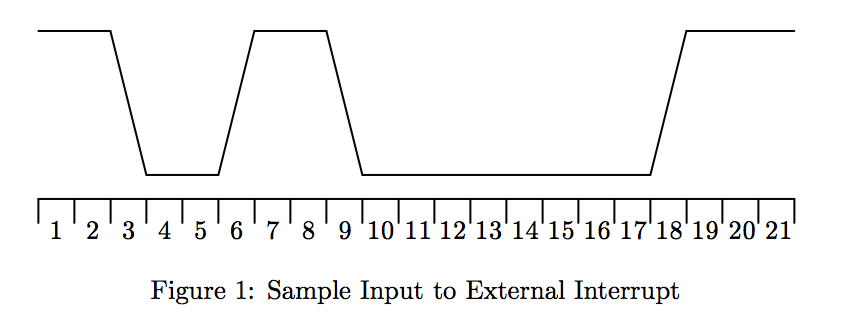
\includegraphics[width=0.6\textwidth]{Fig1.png}
		\end{figure}
	
		\begin{itemize}
			 \item 
			 Rising edge detection = \{ (6 - 7), (18 - 19) \}
			 
			 
			 \item 
			 Falling edge detection = \{ (3 - 4), (9 - 10) \}
			 
			 
			 \item 
			 Low level detection = \{ [4 - 6], [10 - 18] \}
			 
			 
			 \item
			High level detection = \{ [0 - 3], [7 - 9], [19 - 22] \}
			
			
		\end{itemize}
		
	\end{enumerate}


\end{document}

